%MIT OpenCourseWare: https://ocw.mit.edu
%RES.18-011 Algebra I Student Notes, Fall 2021
%License: Creative Commons BY-NC-SA 
%For information about citing these materials or our Terms of Use, visit: https://ocw.mit.edu/terms.

\section{Isometries}
\subsection{Review}
Last time, we discussed the orthogonal matrices $O_n$, which are matrices which preserve the dot product, which is a measure of length. We found that if we looked at the orthogonal matrices which had determinant 1, $SO_n,$ they actually turned out to be rotations in 2-space and 3-space! The rest of the orthogonal matrices $O_3$ can be obtained from $SO_3$ by multiplying a rotation matrix by 
\[
\begin{pmatrix}
-1 & & \\
& 1 & \\
& & 1
\end{pmatrix};
\]
the result will be a reflection over some axis. As a result, all length-preserving $3 \by 3$ matrices are rotations or reflections. 

\subsection{Isometries}

Without any prior knowledge, we might assume that there are many different types of length-preserving mappings, called isometries. We found that for linear mappings, the isometries were the orthogonal matrices, and two or three dimensions, they were rotations or reflection. What are the possibilities for isometries that are not linear?

\begin{qq}
Orthogonal matrices are the linear mappings that preserve distance. What are the other possibilities for distance-preserving mappings that are not necessarily linear?
\end{qq}

An isometry from $\RR^n$ to $\RR^n$ is a length-preserving mapping. 

\begin{definition}
A function $f: \RR^n \rto \RR^n$ is an \textbf{isometry} if 
\[
|f(u) - f(v)| = |u - v|
\]
for all $u, v \in \RR^n.$
\end{definition}

Let's take a look at two key examples.

\begin{example}
For a matrix $A \in O_n,$ the linear transformation 
\begin{align*}
\RR^n &\rto \RR^n \\
\vv{x} &\mapsto A\vv{x}
\end{align*}
is an isometry.
\end{example}


\begin{example}
Translation by a vector $\vv{v} \in \RR^n$ \footnote{This is \emph{not} a linear transformation!} is an isometry:
\begin{align*}
    \RR^n &\xrightarrow[]{t_{\vv{b}}} \RR^n \\
    \vv{x} &\mapsto \vv{x} + \vv{b}
\end{align*}
\end{example}

How crazy can an isometry be? The answer, fortunately or unfortunately, is \emph{not very}. In fact, these two examples and their compositions turn out to be the \emph{only} isometries. 

\begin{theorem}\label{isometry linear trans}
Every isometry $f$ is of the form $t_{\vv{b}}\circ A,$ for $A \in O_n$ and $\vv{b} \in \RR^n.$ So $f(\vv{x}) = A\vv{x} + \vv{b}.$
\end{theorem}

Despite the fact that preserving distance does not appear to be a very strong condition on $f$, it turns out that it is equivalent to the very strong condition that it basically has to be linear, combined with a shift. It boils down to the following lemma. What form do the isometries that fix the origin take? The answer is that they must be linear.

\begin{lemma}
If $f: \RR^n \rightarrow \RR^n$ is an isometry such that $f(0) = 0,$ it must be a linear transformation.\footnote{It must respect the additive and scalar multiplicative structure on $\RR^n$.} 
\end{lemma}

\begin{proof}

We must show that $f$ preserves sums and scalar products. First, we see that a dot product can be written in terms of $\vv{0}$ and distances:
    \[
    \vv{u} \cdot \vv{v} = \frac{1}{2}\left(|\vv{u} - \vv{0}|^2 + |\vv{v} - \vv{0}|^2 - |\vv{u}-\vv{v}|^2\right).
    \]
    
As a result, the following equation also holds:
    \[
    f(\vv{u}) \cdot f(\vv{v}) = \frac{1}{2}\left(|f(\vv{u}) - f(\vv{0})|^2 + |f(\vv{v}) - f(\vv{0})|^2 - |f(\vv{u})-f(\vv{v})|^2\right).
    \]
    
    Because $f$ is an isometry, $|a-b| = |f(a)-f(b)|$. Setting $f(0) = 0$ gives the equation $\vec{u} \cdot \vec{v} = f(\vec{u}) \cdot f(\vec{v}),$ so it must be the case that since $f$ preserves lengths, $f$ also preserves the dot product.
\begin{itemize}
    \item The sum can be expressed using a dot product again. For $\vv{z} = \vv{x} + \vv{y},$ 
    \[
    (\vv{z} - \vv{x}-\vv{y}) \cdot (\vv{z} - \vv{x}-\vv{y}) = 0,
    \]
    and so 
    \[
    \vv{z} \cdot \vv{z} + \vv{x} \cdot \vv{x} + \vv{y}\cdot\vv{y} - 2\vv{x}\cdot\vv{z} - 2\vv{y}\cdot \vv{z} + 2\vv{x}\cdot\vv{y} = 0.
    \]
    
    Now, since we know that addition is determined in some complicated way from dot product, since $f$ fixes the dot product, it must fix addition as well. \footnote{If we had some other crazy invented operation determined from the dot product, $f$ must also fix that!}
    So $f(z) = f(x) + f(y).$
    
    \item A similar reasoning gives us the scaling product: $f(cx) = cf(x).$
\end{itemize}

\end{proof}

Despite the fact that the only piece of information is that $f$ preserves distances and maps the origin to itself, it is enough to play around algebraically to find out that $f$ must be linear. This rules out lots of crazy functions that you could imagine could be isometries. 

\begin{proof}[Proof of Theorem \ref{isometry linear trans}]


Now, we can prove the original theorem. Given $f: \RR^n \rto \RR^n,$ there is some vector $b \in \RR^n$ such that $f(0) = b.$ Then $t_{-b} \circ f$ is an isometry that fixes $0.$ Thus, there is some linear transformation $A$ such that $t_{-b} \circ f = A,$ and this implies that $f = t_{b} \circ A,$ since $t_{b}$ is the inverse of $t_{-b}.$ From the definition of an isometry, it is easily seen that the composition of two isometries is an isometry.

\end{proof}

Given that isometries are all of the same restrictive form, it is not surprising that they form a group.

\begin{definition}
The \textbf{group of isometries} is
\[
M_n \coloneqq \{\text{isometries } \RR^n \xrightarrow[]{f} \RR^n\} \subseteq \text{Perm}(\RR^n).\footnote{Any bijective function on $\RR^n$ permutes the vectors in $\RR^n,$ since it maps each vector in $\RR^n$ to exactly one vector in $\RR^n,$ which is potentially itself.}
\]
\end{definition}

Clearly, translations, which are isomorphic to $(\RR^n, +),$ form a subgroup of $M_n,$ since $t_{\vv{b}} + t_{\vv{b'}} = t_{\vv{b}+\vv{b'}}$. Orthogonal matrices $O_n$ also form a subgroup of $M_n.$

Note that the composition of an orthogonal matrix with a translation is
\[
A\circ t_{\vv{b}} = t_{A\vv{b}} \circ A,
\]
since 
\[
A(x + b) = Ax + Ab. 
\]
In particular, a translation and an orthogonal matrix do \emph{not} commute with each other.

Consider the projection \begin{align*} \pi: &M_n \rto O_n \\
& t_b \circ A \mto A.\end{align*} 
It is a group homomorphism, since 
\[
(t_b \circ A) \circ (t_{b'} \circ A') = t_{b + Ab'} \circ AA'.
\]
Also, $\pi$ is surjective, and the kernel is $\ker(\pi)$, which are translations. Thus, the subgroup of translations is normal inside $M_n.$

\subsection{Isometries in 2-space}

Now that we have an understanding of isometries in general, let's narrow it down to an analysis in two dimensions.

\begin{qq}
For $n=2$, what do isometries look like?
\end{qq}

The following definition is an intuitive extension of the idea of orientation for linear mappings.

\begin{definition}
An isometry $x \mapsto Ax + b$ is \textbf{orientation-preserving} if $\det(A) = 1$, and \textbf{orientation-reversing} if $\det(A) = -1.$
\end{definition}

In two dimensions, isometries can be classified into one of four types.
\begin{theorem}\label{isometry four}
Every isometry on $\RR^2$ is 
\begin{enumerate}
    \item Translation
    \item Rotation around a point $p$\footnote{It is no longer required that $p$ is the origin, since the isometry does not have to be a linear transformation}
    \item Reflection across a line $L$ \footnote{Again, the line $L$ may or may not pass through 0; the isometry is not necessarily linear.}
    
    \begin{center}
        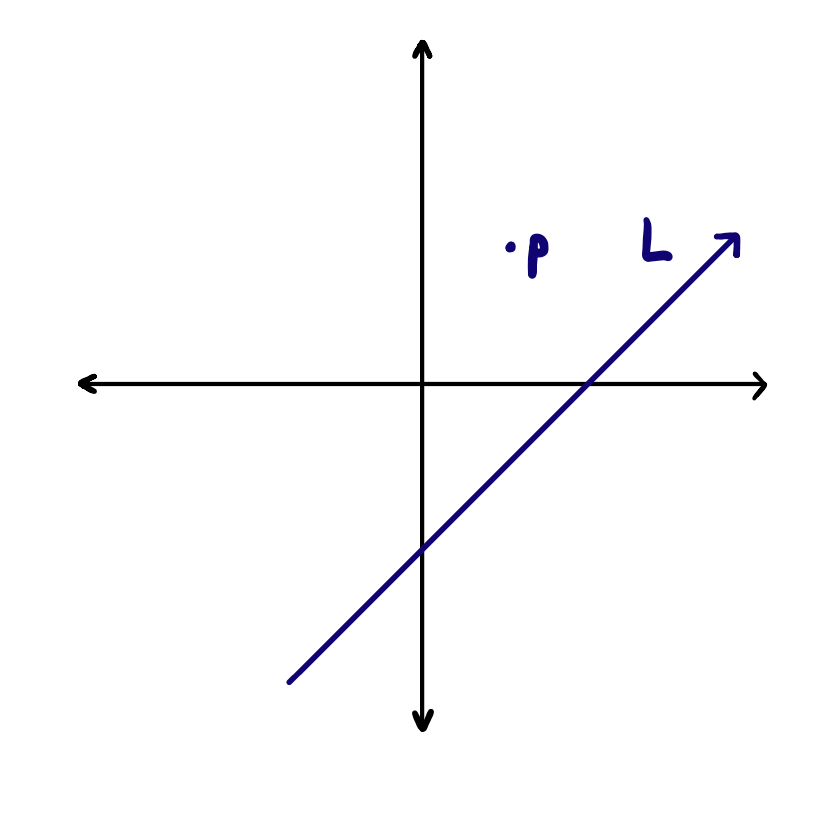
\includegraphics[width=5cm]{Lecture Files and Images/lec13-1a.png}
    \end{center}

    \item Glide reflection --- first, reflect across a line $L,$ then translate by some vector $b$ parallel to $L$\footnote{We will see diagrams next week which have glide reflections in their symmetry group!}
\end{enumerate}
\begin{center}
 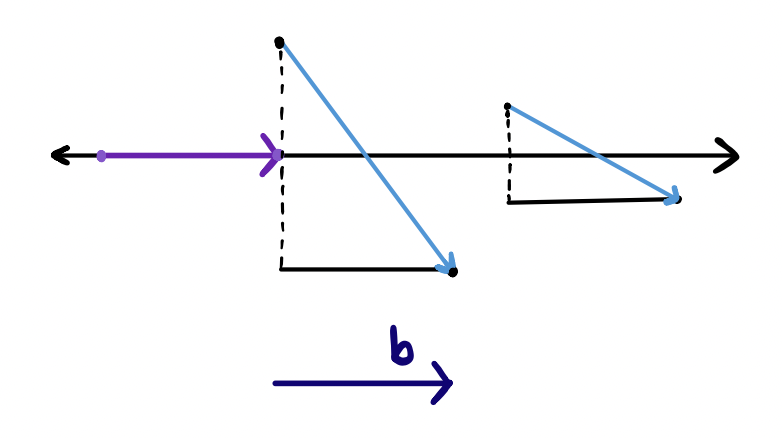
\includegraphics[width=5cm]{Lecture Files and Images/lec13-1b.png}
\end{center}
\end{theorem}

The first two are orientation-preserving; the last two are orientation-reversing. 

By composing with translations, it is possible to essentially change coordinate systems. For example, consider rotations and reflections. Let $f$ be an isometry, say a rotation around the origin. Then, 
\[
t_p f t_{-p}
\]
is a new isometry that fixes $p$, instead of the origin, since it is applying $f$ but after shifting coordinates by $p.$ \footnote{When we apply $t_{-p}$, we shift $p$ to 0, then we use $f$ to rotate around 0, and lastly use $t_p$ to shift $0$ back to $p.$} 

Similarly, letting $f$ be a reflection across any line, we can represent it in new coordinates as a reflection across a line through the origin. 

\begin{proof} We split the proof up into two cases depending on whether $f$ is orientation-preserving or reversing.
\begin{itemize}
    \item 
\textbf{Case I.}
Consider an orientation-preserving isometry $f(x) = A_{\theta}x + b.$  %37:16???

\begin{enumerate}
    \item If $A_{\theta} = I_2$, the identity, then $f = t_b,$ which is possibility 1 in the theorem.

    \item Otherwise, if $A_{\theta} \neq I_2,$ we want to find a fixed point $p$ such that $f(p) = p.$ Since $A_{\theta}$ has no fixed vectors, $p_A(1) \neq 0,$ and so $A_{\theta} - I_2$ has a trivial kernel, and so $A - I_2$ is invertible. Then the equation 
\[
(A-I_2) p = -b
\]
has a unique solution $p = (A-I_2)^{-1}(-b),$ and then 
\[
f(p) = Ap + b = p.
\]
So 
\[
t_{-p} A t_p = A_{\theta},
\]
since it fixes 0. This corresponds to the second possibility: rotation around a point $p.$
\end{enumerate}

\item \textbf{Case II.} 


Let $f$ be an orientation-reversing isometry. Then $f = t_b \circ A,$ where $A$ is reflection across a line $L.$ First, change the origin to $b/2.$ Then 
\[
t_{-b/2} f t_{b/2} = t_{-b/2} t_b A t_{b/2} = t_{b/2} t_{Ab/2} A = t_m A,
\]
where $m = \frac{b + Ab}{2}.$ Since $b$ and $Ab$ are reflections over a line $L,$ $m$, the average, must lie on that line. 
\begin{center}
    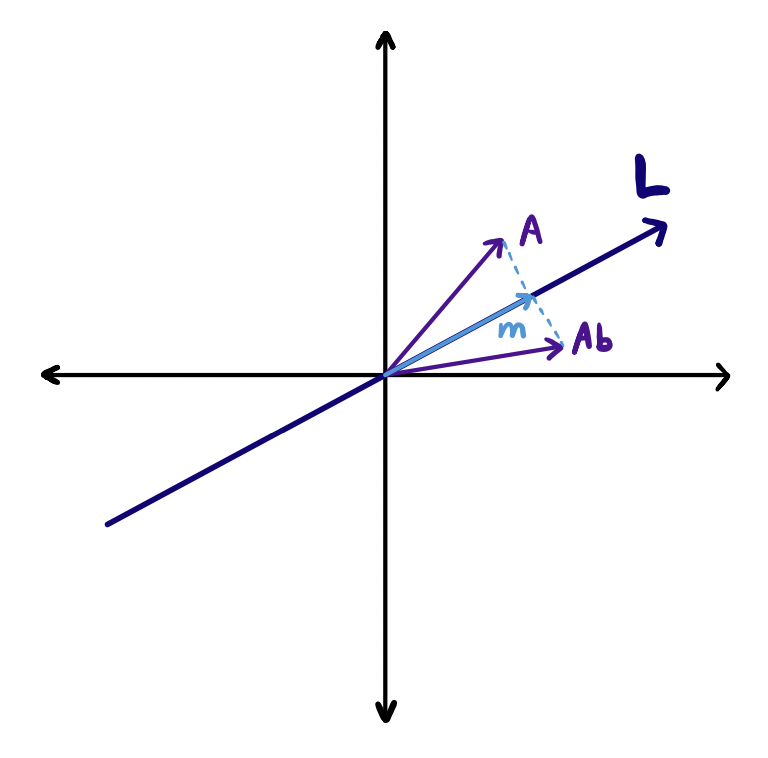
\includegraphics[width=8cm]{Lecture Files and Images/lec13-2alt.png}
\end{center}

\begin{enumerate}
    \setcounter{enumi}{2}
    \item If $m = 0,$ it is a reflection. 
    \item If $m \neq 0,$ it is a glide reflection. \footnote{In our proof, we try to be slicker about it, but if we are uncomfortable with that, we know $f$ is just $Ax + b,$ and we could simply crunch through lots of sines and cosines to force $f$ into one of the four forms in Theorem \ref{isometry four}.}

\end{enumerate}

Again, the same idea from Case I applies. Shifting to a new coordinate system gives us either a reflection or a glide reflection.

\end{itemize}

\end{proof}


\newpage